\documentclass[10pt]{article}
\usepackage[preprint]{tmlr}
\usepackage[hidelinks,pdfstartview={}]{hyperref}
\usepackage{url}
\usepackage{booktabs}
\usepackage{etoolbox}
\AtBeginEnvironment{table}{\setlength{\belowcaptionskip}{6pt}}
\usepackage{amsmath,amssymb}
\usepackage{graphicx}
\usepackage{xcolor}
\usepackage{microtype}
\usepackage{enumitem}
\usepackage{multirow}
\usepackage[capitalise,noabbrev]{cleveref}
\setlist{itemsep=2pt,topsep=3pt}

\newcommand{\alive}{\textsc{alive}}
\newcommand{\dead}{\textsc{dead}}

\title{HALF-LIFE: Forecasting When Visual Memories\\Stop Being True}

\usepackage[T1]{fontenc}
\author{Yixuan Yang\\Independent researcher}
\begin{document}
\maketitle

\begin{abstract}
An agent that observes a scene intermittently must decide which remembered observations are still current: a person's posture can change within seconds while their clothing persists. We study \emph{endpoint validity forecasting}: given a textual memory built from past video and a gap~$\Delta$, predict the probability that a remembered statement still holds at $t+\Delta$. Two-sided supervision comes automatically from fixed-camera Ego-Exo4D video: later captions confirm statements, and a visual interrogator labels unconfirmed ones as still true, no longer true or undeterminable, so silence never counts as invalidity. A LoRA-adapted text-only forecaster (Qwen3.8-27B) outperforms counting, ridge and gradient-boosted baselines on held-out recordings and, on 31 further confirmation recordings, beats counting and contextual ridge at every gap, including one never used in training. On the confirmation recordings, the same model prompted without adaptation already forecasts but, with calibrated scores, falls between those two baselines in every cell: on volatile statements (defined operationally by low re-emission) at 120\,s, Brier score is 0.156 for counting, 0.139 for the prompted model, 0.126 for contextual ridge and 0.112 for the adapted forecaster. Adaptation also improves discrimination: when 5\% of valid volatile statements may be rejected, the forecaster catches 51\% of the invalid ones at 120\,s, against 39\% for contextual ridge and 20\% for the prompted model. Used to select memory for a caption generator, the forecasts beat no memory under an automatic visual judge and show suggestive gains over contextual-ridge selection: most point estimates favor the Forecaster, including the human-reference-assisted comparison, while the confidence intervals include zero. Memory validity is learnable from automatically labeled video, and adaptation adds to what prompting the same model achieves; the downstream results offer early evidence that these forecasts can help select useful memory.
\end{abstract}

\section{Introduction}
\label{sec:intro}

At one moment in a kitchen video, an observer records two facts: \emph{a person is crouching behind a kitchen island} and \emph{the person is wearing a white long-sleeved top and glasses}. Both were last mentioned half a second earlier and both appeared in 3.7\% of the recent observation windows. Two minutes later the person is standing at the counter, still in the same clothes. Equal recency does not imply equal reliability: a memory system should keep trusting the clothing and treat the posture as a candidate for re-observation.

\Cref{fig:example} shows this case from our confirmation data. A counting baseline built from content words and elapsed time assigns both statements a probability above 0.86 of still holding. Our learned forecaster assigns 0.083 to the posture and 0.997 to the clothing. The example captures the question behind HALF-LIFE: \emph{can the validity of a visual memory be learned from its content and context, rather than approximated by a decay rule?}

Memory systems for language and video agents decide what to store, retrieve, consolidate or forget, typically guided by recency, importance or a forgetting curve \citep{packer2023memgpt,zhong2024memorybank}. Long-video models compress or stream past observations \citep{song2024moviechat,he2024malmm,chen2024videollmonline}, and robot memories index what was seen and where \citep{anwar2024remembr}. These systems organize historical evidence, while recent work also detects or revises stale memories using new observations or action records \citep{chao2026stale,sun2026memorylies,wang2026oldisnotfalse}. We ask what can be predicted while observation is suspended: a retrieved statement can describe the past accurately yet have uncertain validity at a later time. A forecast of that validity can guide which memories to trust or refresh, without generating future images or locating the exact moment a fact changed.

We formulate this as binary probabilistic prediction at a requested future time. A frozen vision--language Observer turns recent clips into text; a data builder forms a memory inventory from past observations only; future video supplies the label for one queried statement, through either textual entailment from a later caption or a targeted visual Interrogator; and a text-only Forecaster learns the map from the past memory and a gap to a validity probability. Video thus provides temporal supervision, while the learned predictor operates on a language memory that is available when observation is suspended.

We ask three questions in turn. Can validity be learned from automatically labeled video better than by decay rules and feature models? Does supervised adaptation add anything beyond prompting the same language model with the same input? And does a better validity forecast change a downstream decision, here which remembered facts accompany a caption generator?

\begin{figure}[t]
\centering
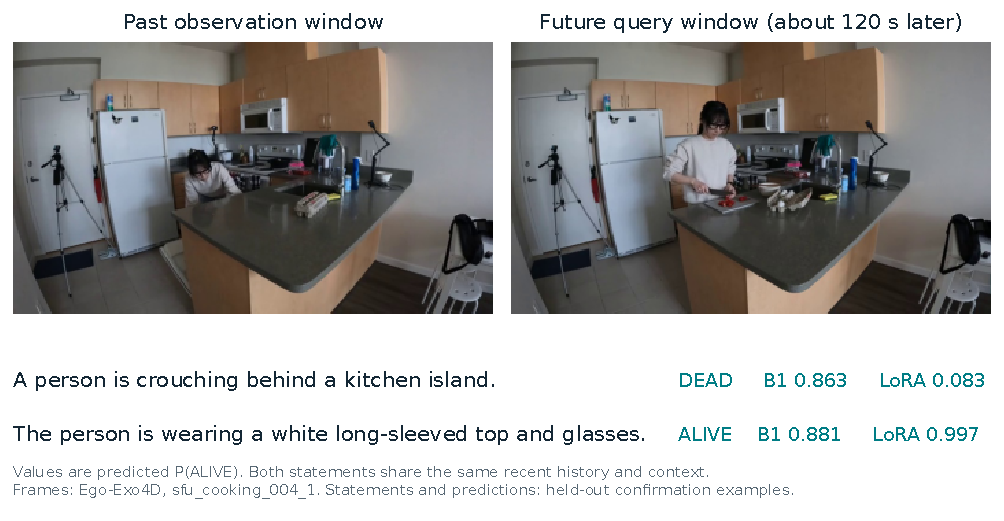
\includegraphics[width=0.94\linewidth]{figures/halflife_fig1_example.pdf}
\caption{\textbf{Two memories with identical recency and mention history have opposite futures.} Past and future frames come from a held-out confirmation recording (Ego-Exo4D, \texttt{sfu\_cooking\_004\_1}); only the past-derived text enters the Forecaster, and the future frames supply the labels. Values are predicted P(\alive) at a 120\,s gap. The counting baseline (B1) rates both statements as likely to persist; the Forecaster (LoRA) separates the transient posture from the persistent clothing.}
\label{fig:example}
\end{figure}

\paragraph{Contributions.}
\begin{itemize}
\item \textbf{A task and an automatic labeling pipeline.} We define endpoint validity for perceptual memories and construct two-sided labels from video by combining caption entailment with targeted interrogation that has an explicit \emph{cannot tell} outcome. The pipeline yields 62,162 labeled statement--gap pairs on 95 recordings, with a measured error profile (\cref{sec:labels}).
\item \textbf{A forecaster that learns which memories go stale.} A LoRA-adapted language model beats a ladder of increasingly informed baselines on held-out recordings, and the counting and contextual-ridge baselines on a second confirmation cohort and at an untrained gap. With calibrated scores, the same model prompted without adaptation falls between those two baselines on the confirmation cohort, and adaptation improves on it at every gap, with raw and with separately calibrated scores. At a fixed 5\% false-rejection rate of valid statements, the adapted model catches more invalid statements than contextual ridge and the prompted model at every gap (\cref{sec:results}).
\item \textbf{A downstream test of utility.} Captions written with forecast-selected memory are preferred over captions without memory by an automatic visual judge. Comparisons with contextual-ridge selection show suggestive gains: most point estimates favor the Forecaster, including the human-reference-assisted comparison, while all corresponding confidence intervals include zero (\cref{sec:captioning}).
\end{itemize}

\section{Related work}
\label{sec:related}

\paragraph{Memory for language agents.} MemGPT moves information between memory tiers to extend an LLM's usable context \citep{packer2023memgpt}; MemoryBank combines retrieval with a forgetting mechanism driven by elapsed time and memory significance \citep{zhong2024memorybank}; LongMemEval tests temporal reasoning, knowledge updates and abstention over long interaction histories \citep{wu2025longmemeval}. These works study storage, retrieval and update-sensitive evaluation. Our task estimates the probability that a perceptual statement remains valid after a specified interval with no new evidence available to the predictor. Our B1 baseline is a task-fitted content-and-time decay model in the spirit of forgetting curves, not a reproduction of any of these systems.

\paragraph{Long-video and embodied memory.} Long-video models maintain compressed or streaming memories \citep{song2024moviechat,he2024malmm,chen2024videollmonline}, Ego4D's episodic-memory tasks localize answers in past video \citep{grauman2022ego4d}, and ReMEmbR builds a long-horizon spatio-temporal memory for robot navigation \citep{anwar2024remembr}. These works retrieve or summarize the past. Our target is the validity of an existing textual assertion at a later time, which is complementary: it can rank or gate what such memories return. We use selected fixed third-person views from Ego-Exo4D \citep{grauman2024egoexo4d}, where a static camera makes later verification practical.

\paragraph{Temporal validity of facts.} A closely related predictive formulation comes from text. \citet{zhang2023mitigating} predict how long a fact will remain true and use the prediction to discard outdated facts in question answering; time-sensitive QA evaluates answers that change over time \citep{chen2021timesensitive}; temporal commonsense benchmarks probe typical event durations \citep{zhou2019going}. HALF-LIFE moves the question from encyclopedic facts to perceptual statements about a scene, where validity is decided by later video, can be unobservable, and depends on the surrounding activity.

\paragraph{Detecting and revising stale memories.} STALE evaluates whether an agent revises a stored belief when later dialogue implicitly invalidates it \citep{chao2026stale}. SpatialSTALE tests conflicts between spatial memories and current observations in a dynamic grid environment, including their consequences for navigation \citep{sun2026memorylies}. ReDate assigns valid times to retrieved visual memories using an action log, including cases where a scene returns to an earlier state \citep{wang2026oldisnotfalse}. These studies establish memory validity as a distinct issue beyond retrieval and recency. HALF-LIFE addresses a complementary information setting: after observation stops at $t$, the predictor receives only past-derived text and a requested gap, with no intervening observation or action log. It forecasts endpoint validity probabilistically from automatically labeled real video. The learned probabilities can then guide memory selection for a downstream caption generator.

\paragraph{Probabilistic evaluation.} We train with LoRA \citep{hu2022lora} and read probabilities from the likelihoods of two fixed answers, in the spirit of \citet{kadavath2022language}. Brier score is a strictly proper scoring rule \citep{brier1950verification,gneiting2007strictly}; we use isotonic post-processing \citep{zadrozny2002transforming}, report calibration error \citep{guo2017calibration}, and use Murphy's decomposition \citep{murphy1973new} to separate reliability from resolution; discrimination is read from ROC operating points at fixed false-rejection rates.

\section{Endpoint validity from video}
\label{sec:labels}

\subsection{Prediction target}
Let $t$ be an observation anchor, $\mathcal{C}_t$ a textual memory constructed from observations no later than $t$, $s \in \mathcal{C}_t$ a queried statement, and $\Delta > 0$ a requested gap. The forecaster estimates
\begin{equation}
p_\theta(s,t,\Delta) = P\big(Y(s,t+\Delta)=1 \mid \mathcal{C}_t, s, \Delta\big),
\label{eq:target}
\end{equation}
where $Y=1$ means that the evidence at the endpoint supports the statement and $Y=0$ that it supports its invalidity. Endpoints whose evidence is visually unresolved are excluded from training and evaluation. This is \emph{endpoint} validity: a statement may become false and later true again, no monotonicity is imposed across gaps, and we do not estimate the time of first invalidation. \alive{} and \dead{} are the model's two answer strings, not categories of objects; a persistent object can take part in an invalid relation, as when vegetables remain in the kitchen after ``the vegetables are on the cutting board'' becomes false.

\subsection{Memory from past observations}
For each recording, a frozen vision--language Observer describes three-frame clips spanning about two seconds, with observation windows sampled at 2\,Hz. Its outputs separate visible statements, motion descriptions and inferred activity context; short clips let the description capture transitions such as a person lowering their body.

At anchor $t$, candidate facts are collected from the most recent second of Observer output, deduplicated and capped at 12. For each candidate $s_i$ we summarize the preceding 30 seconds by its last-mention age $a_i$ and its mention fraction $f_i$, using lexical matching to recent descriptions. Note that $f_i$ measures how often the Observer \emph{mentioned} a statement, not how long it was true. The forecaster's input is a text sequence containing (i) the inventory of statements with $a_i$ and $f_i$, (ii) the last-observed motion and inferred context for the queried statement, (iii) the requested gap and (iv) the queried statement. No future caption, interrogation answer or frame enters the input, so the representation is available at inference while observation is suspended.

\subsection{Two-sided endpoint labels}
\label{sec:twosided}
Silence is not evidence of change: a later description that fails to mention a fact does not show that it became false. We therefore use a two-route cascade. At $t+\Delta$, a later description that entails $s$ under a fixed natural-language-inference matcher supplies a positive label. Otherwise, the Interrogator (the Observer's checkpoint with a different prompt) examines a three-frame window around the endpoint and answers \textsc{still-true}, \textsc{no-longer-true} or \textsc{cannot-tell}, mapped to $Y=1$, $Y=0$ and a masked row. Occlusion and ambiguity can make a decision impossible, which is why the unknown outcome is kept rather than forced into a class.

Across the original 64-recording universe, 50,320 candidate pairs yield 48,506 usable rows (22,783 positive entailment labels and 25,723 Interrogator labels) and 1,814 masked rows. The 31-recording confirmation universe yields 13,656 usable rows (6,575 entailment, 7,081 Interrogator) and 588 masked rows from 14,244 candidates. All negative labels come from direct visual interrogation.

\subsection{Label quality}
The labels are automatic measurements, so we characterize their error. On blind reference sets judged with AI-assisted frame inspection and partial human spot checks, the false-valid rate is 20.8\% [10.4\%, 32.6\%] among 48 adjudicable reference-invalid items, and the false-invalid rate is 4.3\% among 47 reference-valid items. In other words, about one in five reference-invalid statements is labeled valid, while false invalidity is rare. Confirmation labeling also passed pre-specified consistency controls: 13 of 200 cross-recording control queries were accepted as valid (6.5\%, threshold $\le$10\%), and a blind drift check agreed on 23 of 27 adjudicable items (85.2\%, threshold $\ge$80\%). We train and evaluate on the resulting hard labels without noise correction; \cref{sec:limitations} discusses what this implies.

\section{Forecaster and baselines}
\label{sec:method}

\subsection{Supervised adaptation and scoring}
The Forecaster is Qwen3.8-27B \citep{qwen2026qwen38} used as a text-only model; the visual stage of the pipeline has already produced the memory text. We train rank-16 LoRA adapters (scaling 32, dropout 0.05) for one epoch on 20,119 examples from 33 fit recordings, with supervised gaps $\Delta \in \{8, 32, 120\}$\,s; the 64\,s gap is excluded from training and used to test interpolation. AdamW with learning rate $10^{-4}$, a cosine schedule and effective batch 16 gives 1,258 optimizer steps. The prompt contains the memory and query; the target is \alive{} or \dead{}, trained with autoregressive cross-entropy on the answer while prompt tokens are masked from the loss. No verbal rule such as ``postures are short-lived'' is supplied: any regularity must be learned from the association between memories and endpoint labels.

At evaluation both candidate answers are teacher-forced. With $z_1$ and $z_0$ the summed log-likelihoods of the two answers,
\begin{equation}
\hat p_{\text{raw}} = \frac{\exp(z_1)}{\exp(z_1)+\exp(z_0)} = \sigma(z_1 - z_0).
\label{eq:score}
\end{equation}

\subsection{Baselines}
The baselines form a ladder of increasingly informed predictors, each answering a question about where the signal lies.
\begin{itemize}
\item \textbf{B0, gap base rate:} the fit-population positive frequency at each gap. \emph{How far do class imbalance and elapsed time alone go?}
\item \textbf{B1, content-and-time counting:} for each content word $w$ and trained gap $d$, with $n_{wd}$ examples containing $w$, $k_{wd}$ of them positive, and gap base rate $p_{0d}$, a smoothed rate $q_{wd} = (k_{wd} + 20\,p_{0d})/(n_{wd}+20)$ over words with $n_{wd}\ge 20$. A statement's prediction averages its word rates (falling back to $p_{0d}$); 64\,s is interpolated in log time. \emph{Does content-specific decay explain validity?}
\item \textbf{B2, lexical ridge:} ridge regression on statement bag-of-words, mention fraction, normalized last-mention age and log gap. \emph{Do learned weights over words and observation history suffice?}
\item \textbf{B3, contextual ridge:} B2 plus sentence embeddings \citep{reimers2019sentence,wang2020minilm} of the statement and of its last-seen visible, motion and context descriptions, each projected to 24 dimensions on fit data. \emph{Does lightweight context explain the gain?}
\item \textbf{B4, nonlinear features:} histogram gradient-boosted trees on B3's features. \emph{Does a nonlinear model over the same features close the gap?}
\item \textbf{Prompted base:} the Forecaster's checkpoint without the adapter, with the identical past-only input, gap request, chat format and two-answer likelihood readout (\cref{eq:score}), and with no prompt search or training. \emph{How much of the Forecaster's skill does the pretrained model already provide when prompted?}
\end{itemize}
The feature ladder spans increasingly informative inputs; it is not an ablation of the Forecaster's inputs. The prompted base isolates adaptation: it shares the Forecaster's model and input and differs only in the adapter.

\subsection{Calibration}
B2, B3, B4, the prompted base and the Forecaster each receive their own monotone map, fitted by pool-adjacent-violators on the same deterministic 11,050-row train-side subset at the three supervised gaps \citep{zadrozny2002transforming}; B0 and B1 use their counting estimates directly. No evaluation label is used for calibration. The maps are nondecreasing, so they never reverse the order of two scores, but they can merge scores into ties and therefore change AUC slightly. Because a good ranking need not have the right probability scale, and a calibration map need not improve out-of-population Brier score, we report both calibrated and raw results.

\section{Experimental setup}
\label{sec:setup}

\paragraph{Recordings and splits.} The study uses 95 labeled Ego-Exo4D recordings (``takes''): an original universe split into 33 fit and 31 internal held-out takes, plus 31 additional confirmation takes. Splits group related takes by capture and participant so that no group crosses the fit/evaluation boundary. The internal held-out set contains 21,711 scored rows and the confirmation set 13,656. No predictor, baseline or calibration map is fitted to confirmation labels. The prompted base is scored on all 62,162 usable rows, which include both evaluation sets and the 11,050-row calibration subset; these are matched evaluations, not independent test cases. The confirmation takes were scored once by an earlier implementation before a repair to input construction; the results reported here re-evaluate them under the fixed protocol with the corrected implementation.

\paragraph{Populations.} We report all statements and a pre-declared \emph{volatile} stratum, defined operationally by low re-emission: statements whose content-word counting estimate of 120\,s caption re-emission is below 0.5419, the median over unique statements in the original universe. The stratum is fixed before Forecaster training and reused unchanged on the confirmation takes. It is a proxy for low re-emission, not a measurement of physical instability: in the confirmation set, 971 of 5,687 volatile rows are \dead{} (17.1\%) against 240 of 7,969 other rows (3.0\%). The stratum therefore concentrates the harder prediction problem while retaining many positive outcomes.

\paragraph{Metrics.} The primary metric is take-macro Brier score, which weights each take equally so that long recordings do not dominate:
\begin{equation}
\mathrm{BS}_{\text{macro}} = \frac{1}{|V|}\sum_{v\in V}\frac{1}{|I_v|}\sum_{i\in I_v}(\hat p_i - y_i)^2 .
\end{equation}
Differences are baseline minus Forecaster Brier, so positive values favor the Forecaster. Paired 95\% intervals use 10,000 bootstrap resamples of capture groups, retaining the takes within each group, and we count the takes that improve. Expected calibration error (ten equal-width bins) and AUC use pooled rows.

\paragraph{Discrimination at a fixed false-rejection rate.} Brier score mixes discrimination with the probability scale. To measure how well a predictor separates invalid from valid statements, we also report the fraction of invalid (\dead{}) statements that a predictor rejects when its threshold rejects a fixed fraction (5\% or 10\%) of valid statements, read from the empirical ROC of the raw prompted-base and Forecaster scores and of the saved B3 probabilities. B3 has tied scores, so an exact rate is obtained by linear interpolation between ROC points, which is equivalent to randomized rejection at the boundary score (\cref{app:results} gives the deterministic alternative). Paired 95\% intervals resample the same 24 capture groups for all methods (2,000 resamples) and are pointwise, without adjustment across cells. These operating points are retrospective diagnostics of the confirmation predictions, not thresholds validated on a separate cohort.

\paragraph{Pre-specified confirmation criteria.} Against both B1 and B3 on volatile statements at the three trained gaps, at least two gaps must show a positive bootstrap interval and an improvement on at least 60\% of takes; a third criterion compares against B3 on Interrogator-negative rows pooled over gaps. All three criteria pass. The checkpoint is a single training run, so intervals quantify variation across recordings rather than across training seeds.

\section{Results}
\label{sec:results}

\subsection{Forecasting transfers to new recordings}

\begin{table}[t]
\centering
\caption{\textbf{The Forecaster has the lowest Brier score at every gap in both populations on 31 confirmation takes, and the same model without adaptation falls between counting and contextual ridge.} Take-macro Brier (lower is better), calibrated scores; B1 uses its counting estimates. The 64\,s gap was never used in training. Paired intervals for the volatile rows are in \cref{tab:contrasts,tab:adapt}.}
\label{tab:main}
\begin{tabular}{llrrrrr}
\toprule
Population & Gap (s) & Rows & B1 counting & Prompted base & B3 contextual ridge & Forecaster \\
\midrule
All & 8 & 3,459 & 0.0670 & 0.0624 & 0.0570 & \textbf{0.0508} \\
All & 32 & 3,414 & 0.0849 & 0.0725 & 0.0668 & \textbf{0.0572} \\
All & 64 & 3,411 & 0.0908 & 0.0806 & 0.0743 & \textbf{0.0641} \\
All & 120 & 3,372 & 0.0970 & 0.0864 & 0.0789 & \textbf{0.0692} \\
\midrule
Volatile & 8 & 1,458 & 0.1131 & 0.1054 & 0.0995 & \textbf{0.0853} \\
Volatile & 32 & 1,420 & 0.1373 & 0.1193 & 0.1117 & \textbf{0.0933} \\
Volatile & 64 & 1,424 & 0.1464 & 0.1290 & 0.1195 & \textbf{0.0998} \\
Volatile & 120 & 1,385 & 0.1559 & 0.1392 & 0.1264 & \textbf{0.1116} \\
\bottomrule
\end{tabular}
\end{table}

\begin{figure}[t]
\centering
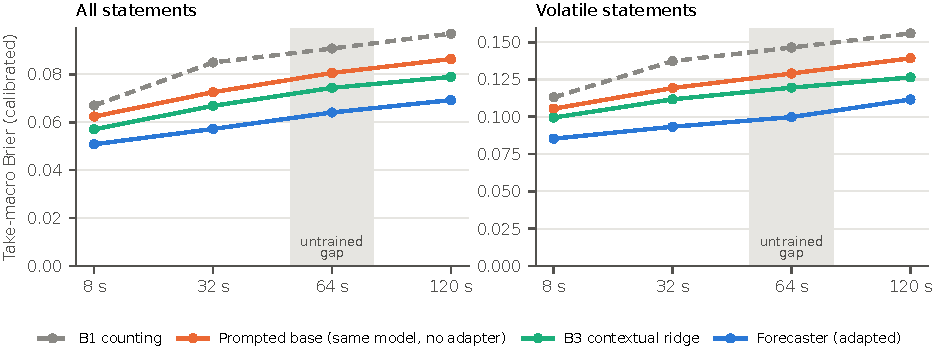
\includegraphics[width=0.96\linewidth]{figures/halflife_fig2_brier.pdf}
\caption{\textbf{The ordering B1 $>$ prompted base $>$ B3 $>$ Forecaster holds at every horizon, including the untrained 64\,s gap.} Calibrated take-macro Brier on the confirmation takes for all statements (left) and the volatile stratum (right). The prompted base is the Forecaster's checkpoint without the adapter. Each method uses one trained predictor at every gap and, if calibrated, one calibration map; B1 uses its counting estimates directly.}
\label{fig:brier}
\end{figure}

\Cref{tab:main} and \cref{fig:brier} report the confirmation results. On volatile statements the Forecaster reduces Brier score relative to B1 by 0.028--0.047 and relative to B3 by 0.014--0.020; all eight population--gap comparisons against each baseline have positive confidence intervals. At 120\,s, volatile Brier falls from 0.1559 (B1) and 0.1264 (B3) to 0.1116, reductions of 0.0443 [0.0287, 0.0623] and 0.0148 [0.0045, 0.0263], with improvements on 28 and 24 of 31 takes. In skill-score terms, the Forecaster removes 28\% of B1's Brier score and 12\% of B3's. At the untrained 64\,s gap it reaches 0.0998, against 0.1464 and 0.1195: performance interpolates to an intermediate horizon without imposing a monotone decay curve. The prompted base, the same model without the adapter, falls between B1 and B3 in all eight population--gap cells.

The internal held-out set also places the Forecaster first (\cref{tab:internal}). At 120\,s on volatile statements, B0 through B4 score 0.2126, 0.1789, 0.1399, 0.1394 and 0.1698, against 0.1166 for the Forecaster. The ladder is informative: learned lexical weights (B2) improve substantially over counting, contextual embeddings in a linear model add almost nothing (B3), and gradient-boosted trees over the same features are worse than the ridge (B4). The adapted language model opens a further gap that these feature models do not close. The comparison establishes the Forecaster as the strongest predictor tested; \cref{sec:adaptation} separates the contribution of adaptation from that of the same model prompted without it.

\subsection{Adaptation improves on the same model prompted without it}
\label{sec:adaptation}

\begin{table}[t]
\centering
\caption{\textbf{Adaptation improves on the same model prompted without an adapter, with raw and with separately calibrated scores.} Confirmation take-macro Brier on volatile statements; gain is prompted base minus Forecaster, with 95\% capture-group bootstrap intervals adjusted for the six primary contrasts (Bonferroni) and the number of takes that improve. The 64\,s gap ($^{\dagger}$) is outside the primary family; its intervals are nominal.}
\label{tab:adapt}
\small
\setlength{\tabcolsep}{3.5pt}
\begin{tabular}{rcccrcccr}
\toprule
& \multicolumn{4}{c}{Raw scores} & \multicolumn{4}{c}{Separately calibrated} \\
\cmidrule(lr){2-5}\cmidrule(lr){6-9}
Gap (s) & Base & Forecaster & Gain [95\% CI] & Takes & Base & Forecaster & Gain [95\% CI] & Takes \\
\midrule
8 & 0.1054 & 0.0846 & 0.0208 [0.0069, 0.0379] & 26/31 & 0.1054 & 0.0853 & 0.0201 [0.0057, 0.0380] & 22/31 \\
32 & 0.1452 & 0.0937 & 0.0515 [0.0263, 0.0726] & 25/31 & 0.1193 & 0.0933 & 0.0260 [0.0131, 0.0395] & 27/31 \\
64$^{\dagger}$ & 0.1736 & 0.0981 & 0.0756 [0.0542, 0.0956] & 29/31 & 0.1290 & 0.0998 & 0.0292 [0.0177, 0.0394] & 26/31 \\
120 & 0.1849 & 0.1087 & 0.0762 [0.0435, 0.1069] & 27/31 & 0.1392 & 0.1116 & 0.0276 [0.0067, 0.0491] & 25/31 \\
\bottomrule
\end{tabular}
\end{table}

The prompted base already carries forecasting signal. Its raw AUC on volatile confirmation statements is 0.79--0.83 across gaps (0.85--0.87 over all statements), and its calibrated Brier score beats counting in every cell. It trails contextual ridge, however, so the pretrained model prompted this way is not what makes the Forecaster the strongest predictor. \Cref{tab:adapt} compares the two directly. Adaptation lowers Brier score at every gap, for raw scores and for separately calibrated ones, and all six primary contrasts (raw and calibrated at 8, 32 and 120\,s) remain positive under the familywise adjustment. At 120\,s the calibrated gain is 0.0276, positive on 25 of 31 takes, against a raw gain of 0.0762: calibration narrows the gap without closing it. Raw AUC rises to 0.88--0.89 at every gap (0.90--0.92 over all statements), so the gain is not only a change of probability scale. The internal held-out set points the same way: at 120\,s on volatile statements, the calibrated prompted base scores 0.1423 against 0.1166 for the Forecaster (\cref{tab:internal}).

\subsection{The Forecaster separates stale from valid memories}
\label{sec:stale}

\begin{figure}[t]
\centering
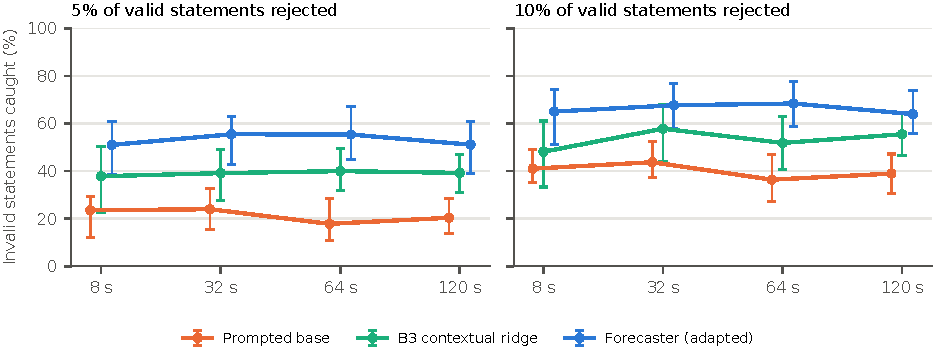
\includegraphics[width=0.96\linewidth]{figures/halflife_fig3_recall.pdf}
\caption{\textbf{At a fixed cost in wrongly rejected valid memories, the Forecaster catches more invalid ones than contextual ridge and the prompted base at every gap.} Fraction of invalid volatile confirmation statements rejected when the threshold rejects 5\% (left) or 10\% (right) of valid ones, from empirical ROC operating points of raw prompted-base and Forecaster scores and saved B3 probabilities; ties are resolved by linear interpolation. Bars are pointwise 95\% capture-group bootstrap intervals. These are retrospective operating points, not validated thresholds; \cref{tab:recall} gives all populations and paired differences.}
\label{fig:recall}
\end{figure}

Most endpoint labels are positive, which makes a high overall validity prior competitive, and Brier score mixes discrimination with the probability scale. We therefore first ask directly how well each predictor separates invalid from valid statements (\cref{fig:recall}). When the threshold rejects 5\% of valid volatile statements, the Forecaster catches 51.0\%, 55.5\%, 55.3\% and 51.1\% of invalid ones at 8, 32, 64 and 120\,s, against 37.8--40.0\% for B3 and 17.8--23.9\% for the prompted base. At 120\,s its advantage is 11.9 percentage points over B3 [1.6, 19.5] and 30.7 over the prompted base [19.1, 40.3]. The Forecaster leads B3 in all sixteen cells (two populations, four gaps, two rates; \cref{tab:recall}), with pointwise intervals above zero. At a fixed cost in valid memories wrongly rejected, the Forecaster identifies more of the memories that have gone stale; this is the evidence that it has learned to recognize them.

\begin{table}[t]
\centering
\caption{\textbf{Outcome-specific Brier describes probability quality given the outcome, and its direction depends on the probability scale.} Confirmation Brier by label route and outcome, pooled over gaps and macro-averaged over eligible takes. ``Entailed positive'': a later caption entails the statement; ``visual'': the Interrogator decided. B1 uses its counting estimates; the other calibrated columns use separately fitted maps.}
\label{tab:route}
\small
\begin{tabular}{lrrrrrrr}
\toprule
& & & \multicolumn{3}{c}{Calibrated} & \multicolumn{2}{c}{Raw} \\
\cmidrule(lr){4-6}\cmidrule(lr){7-8}
Label route and outcome & Rows & B1 & B3 & Base & Forecaster & Base & Forecaster \\
\midrule
Entailed positive & 6,575 & 0.0163 & 0.0190 & 0.0267 & 0.0178 & 0.0667 & 0.0157 \\
Visual positive & 5,870 & 0.0180 & 0.0261 & 0.0334 & 0.0283 & 0.0891 & 0.0248 \\
Visual negative (\dead{}) & 1,211 & 0.6487 & 0.4963 & 0.4764 & \textbf{0.4209} & 0.2883 & 0.4342 \\
\bottomrule
\end{tabular}
\end{table}

\Cref{tab:route} adds probability quality conditional on the outcome. On the 1,211 rows the Interrogator labeled invalid, Brier score is 0.6487 for B1, 0.4963 for B3 and 0.4209 for the calibrated Forecaster; the reduction against B3 is 0.0754 [0.0341, 0.1151], with 23 of 30 eligible takes improving. These are exactly the rows on which positive-caption matching cannot supply a label and a decay rule is most overconfident. The improvement has a price on valid rows: on Interrogator-positive rows the Forecaster scores 0.0283, against 0.0180 for B1 and 0.0261 for B3. The prompted-base columns show why outcome-specific Brier cannot identify the mechanism on its own. With raw scores, adaptation raises invalid-row Brier from 0.2883 to 0.4342 (paired difference $-0.1459$ [$-0.1941$, $-0.0912$]) while lowering it on both valid strata; after separate calibration the invalid-row comparison reverses, to 0.4764 against 0.4209 ($+0.0556$ [0.0055, 0.1128]). Outcome strata respond in opposite directions to the probability scale, so conditional Brier describes probability quality given the outcome, while the fixed-rate analysis above measures discrimination. The paired example in \cref{fig:example}, where only the queried statement changes, shows the separation directly.

\subsection{Calibration and raw scores}
At the 120\,s confirmation endpoint, expected calibration error over all statements is 0.0735 for B1, 0.0107 for B3 and 0.0193 for the calibrated Forecaster (0.0149 raw; \cref{tab:ece}). B3 is better calibrated despite its higher Brier score. The raw Forecaster is already competitive: its Brier at this endpoint is 0.0681 over all statements and 0.1087 over volatile statements, against calibrated values of 0.0692 and 0.1116. Its advantages over the baselines and over the prompted base hold with raw scores as well. Calibration shrinks the gain over the prompted base (on volatile statements at 120\,s, from 0.0762 raw to 0.0276 calibrated) and changes how the Brier gain is distributed across outcomes (\cref{tab:adapt,tab:route}).

\subsection{Robustness to the answer format}
Because \cref{eq:score} scores complete rendered answers, we rescored the same checkpoint on all 62,162 usable rows using only the two label tokens, the label plus end marker, and the full answer, without retraining or refitting any baseline. Removing the end marker and newline changes raw validity probabilities by $1.07\times10^{-7}$ on average internally and $1.01\times10^{-7}$ on confirmation (maximum below $6.7\times10^{-7}$), changes no decision at threshold 0.5, and changes raw Brier by less than $1.4\times10^{-8}$ in every population--gap cell. Formatting tokens do not account for the forecasting performance. Refitting a separate isotonic map for each variant produces slightly larger calibrated differences (mean 0.003), which we trace to tie handling in the isotonic implementation rather than to information in the end marker (\cref{app:tokens}).

\subsection{What individual cases show}
In the crouching/clothing pair, the twelve-fact inventory, motion context, inferred context, recency, mention fraction and gap are identical; only the queried statement changes. The raw Forecaster already separates the two (0.223 vs.\ 0.994) before calibration maps them to 0.083 and 0.997, while B1 gives 0.863 and 0.881. The Interrogator labels the posture invalid and the clothing valid, consistent with the displayed frames. Neither statement belongs to the volatile stratum, which illustrates why statement content, stratum membership and actual outcome should not be conflated.

The same posture statement also exposes a remaining error. Across 8, 32, 64 and 120\,s, its calibrated predictions are 0.370, 0.202, 0.202 and 0.083; the endpoint labels are positive at 8\,s and negative at the other gaps. The model lowers its confidence for more distant postures but is too pessimistic at the shortest gap, a concrete instance of the class trade-off above.

A second kitchen recording shows both a useful contrast and a failure. At a 120\,s gap the model assigns 0.058 to a man still cutting vegetables, 0.993 to a wok remaining on the stove, and 0.800 to chopped ingredients remaining on a cutting board. The first two match the endpoint labels; the third does not, because the person has moved to the sink with an empty board. ``Objects persist, actions change'' is therefore an incomplete rule, and the model's error here is the one that rule would make: object locations and relations also change within an ongoing activity.

\section{Using forecasts to select memory for captioning}
\label{sec:captioning}

Forecasting validity is useful only if a downstream decision can exploit it. We test one such decision with the already-trained Forecaster: which facts from an earlier inventory should accompany current visual input when describing a later scene. The caption generator is not adapted, and the forecasting experiment was not selected for caption performance.

\subsection{Setup}
The no-memory condition V0 receives the current visual input without past facts. V\textsubscript{B3} ranks the available inventory by B3 validity scores and V\textsubscript{LoRA} by Forecaster scores; each keeps $\lceil n/2\rceil$ of $n$ facts within the endpoint's inventory, with deterministic tie-breaking, so the inventory and the number of retained facts match. The comparison therefore tests the value of the ranking under a fixed protocol, not the effect of giving one system more memory. Two caption-generation variants are kept as separate conditions. The automatic evaluation covers 297 endpoints in 24 capture groups: three memory conditions and two variants give 1,782 captions. Two rubrics, applied in both presentation orders, compare V\textsubscript{LoRA} with V\textsubscript{B3} and with V0 (4,752 judgments). The crossed conditions share endpoints and captions, so they are not independent replications.

\subsection{Automatic visual preference}
The judge sees the visual evaluation inputs and two candidate captions. Each preference is canonicalized to $z\in\{-1,0,1\}$, positive favoring the first condition; we average both presentation orders within an endpoint, then endpoints within a capture group, then groups equally:
\begin{equation}
\hat d = \frac{1}{G}\sum_{g=1}^{G}\frac{1}{|E_g|}\sum_{e\in E_g}\frac{z_{e,AB}+z_{e,BA}}{2},
\end{equation}
with 2,000 capture-group bootstrap resamples for intervals. The judge belongs to the same model family as the generator, which limits its independence.

\begin{table}[t]
\centering
\caption{\textbf{Selected memory beats no memory and shows suggestive gains over contextual-ridge selection.} Automatic visual evaluation on the same 297 endpoints in 24 groups. Positive signed preference favors V\textsubscript{LoRA}.}
\label{tab:caption}
\begin{tabular}{llcc}
\toprule
Caption variant & Rubric & LoRA $-$ B3 [95\% CI] & LoRA $-$ V0 [95\% CI] \\
\midrule
1 & Multidimensional & $\phantom{-}0.0486$ [$-0.1284$, 0.2149] & 0.2221 [0.1016, 0.3531] \\
1 & Simple & $-0.0010$ [$-0.1322$, 0.1329] & 0.1780 [0.0675, 0.2846] \\
2 & Multidimensional & $\phantom{-}0.0568$ [$-0.1196$, 0.2312] & 0.1669 [0.0254, 0.3100] \\
2 & Simple & $\phantom{-}0.0048$ [$-0.1316$, 0.1323] & 0.1748 [0.0687, 0.2795] \\
\bottomrule
\end{tabular}
\end{table}

\Cref{tab:caption} shows a benefit of selected memory over no memory: all four LoRA$-$V0 intervals exclude zero. The incremental comparison with B3 shows a positive directional signal: three point estimates favor the Forecaster, including both multidimensional-rubric estimates, while the remaining estimate is near zero. All four intervals include zero, leaving the size and direction of this incremental benefit uncertain.

\subsection{Human-reference-assisted evaluation}
A second protocol gives the model judge sparse human event descriptions as references. It reuses 528 captions and completes 3,722 of 3,744 planned judgments (18 partial, 4 invalid outputs). The primary analysis uses caption variant 2 and 102 references at or before the queried endpoint, covering 61 endpoints in 17 groups; references receive equal weight within annotator, annotators within endpoint, endpoints within group and groups in the final estimate.

\begin{table}[t]
\centering
\caption{\textbf{The positive estimate over B3 persists with human references; intervals span zero.} Signed preference with 95\% capture-group bootstrap intervals; references are sparse event descriptions, not exhaustive scene inventories.}
\label{tab:human}
\begin{tabular}{lrcc}
\toprule
Contrast & Signed preference & 95\% interval & Endpoints / groups \\
\midrule
LoRA $-$ B3 & 0.0618 & [$-0.1267$, 0.2403] & 61 / 17 \\
LoRA $-$ V0 & $-0.1441$ & [$-0.3527$, 0.0809] & 60 / 17 \\
B3 $-$ V0 & $-0.0246$ & [$-0.2333$, 0.1797] & 58 / 16 \\
\bottomrule
\end{tabular}
\end{table}

The positive LoRA$-$B3 estimate persists under this different evaluation protocol, again suggesting potential benefit with substantial uncertainty. The LoRA$-$V0 estimate is negative and its interval spans zero (\cref{tab:human}). A reference can emphasize one event while omitting otherwise useful scene facts, so the two protocols measure different things. Order sensitivity is also substantial: among the 102 primary reference comparisons there are 18 consistent LoRA wins, 10 consistent B3 wins, 14 ties and 60 order-inconsistent pairs.

\subsection{What the application shows}
The application closes the loop from a validity probability to a memory-selection decision, and it locates the open problem precisely. Selected memory helps a caption generator under the automatic visual judge. Relative to contextual-ridge selection, the positive directional signal across most settings suggests that better forecasts can benefit captioning under this fixed retention policy, while the intervals leave the magnitude of the effect uncertain. The pooled fixed-rate analysis does not determine which facts change within a single inventory, where each method keeps half of the facts, so it cannot by itself explain the caption result; the selected facts, the generator's use of them and the judge all intervene between prediction and utility. Closing this gap, for example by training the caption generator to condition on validity estimates or by evaluating decisions that depend on validity more directly, is the most important next step.

\section{Limitations}
\label{sec:limitations}

\paragraph{Labels.} Labels are automatic and come from the same frozen model family as the Observer, which can induce correlated errors. On a small audit, about one in five reference-invalid statements is labeled valid. Reported performance is therefore relative to this labeling instrument on adjudicable examples; better agreement with the instrument does not imply recovery of noise-free physical probabilities, and a disagreement with it is not automatically an error. Resolving this globally requires a broader independent reference set.

\paragraph{Comparisons.} The prompted base uses the Forecaster's prompt without prompt search or few-shot examples, so it is a matched control for adaptation, not a bound on what prompting can achieve. We do not compare other model families or isolate individual context fields, and we do not show that cross-fact reasoning causes the improvement.

\paragraph{Scope.} The study uses fixed third-person cameras in a limited set of skilled activities, one Observer/Interrogator family, horizons from seconds to two minutes, and one adapted-model seed. Transfer to egocentric or mobile viewpoints, other visual models, other activities and longer intervals is untested. Calibration maps are fitted on a subset that overlaps the fit population, and the isotonic implementation is sensitive to tied scores, which is why raw results are reported alongside calibrated ones. The adaptation comparison rests on one adapted checkpoint, the confirmation cohort had been scored before by an earlier implementation, and the fixed-rate operating points are retrospective.

\paragraph{Downstream evidence.} The caption study uses one selection fraction, shared caption sets, model judges and sparse references. It bounds the downstream claim; it does not change the forecasting result. We measure endpoint validity, not task relevance, first-exit time or deployed-agent utility.

\section{Conclusion}
HALF-LIFE formulates memory reliability as endpoint validity: whether a previously observed statement will still hold after a given gap. Labels built automatically from video are enough to train a forecaster that beats content-and-time, lexical, contextual and nonlinear baselines on new recordings and at an untrained horizon. The same model prompted without adaptation already forecasts, but on the confirmation cohort less well than a contextual feature model; adaptation improves probability quality and, at a fixed cost in wrongly rejected valid memories, identifies more of the memories that have gone stale. Using those forecasts to choose memory for captioning helps relative to no memory under the automatic visual protocol; the human-reference-assisted protocol does not establish that contrast. Comparisons with contextual-ridge selection show a positive directional signal in most settings, including the human-reference-assisted comparison, while confidence intervals remain compatible with zero. Memory validity is learnable from automatic video labels, and the downstream results offer early evidence that these forecasts can help select useful memory.

\section*{Broader impact statement}
Validity estimates can make agents that observe people more cautious about acting on outdated observations. The same capability supports persistent visual memory of people, which raises privacy concerns in deployment; our experiments use a consented research dataset and release no raw video.

\bibliography{references}
\bibliographystyle{tmlr}

\clearpage
\appendix

\section{Implementation and data details}
\label{app:impl}

\paragraph{Sampling and eligibility.} The working collection contains 883 downloaded takes, of which 207 have Observer descriptions and 95 contribute labeled data. A take is a continuous activity recording and yields many queries. Anchors are spaced 21\,s apart and require complete observation coverage from $t-1$ through $t+121$\,s; each anchor supplies at most 12 inventory statements queried at four gaps, i.e.\ at most 48 candidate rows before unknown-label masking. The coverage requirement makes the 120\,s target possible, and no endpoint is extrapolated beyond the recording.

\paragraph{Model.} The Forecaster loads the public Qwen3.8-27B checkpoint (64 layers, hidden size 5,120, a hybrid stack repeating three linear-attention layers followed by one full-attention layer) and uses only its text path.

\paragraph{Adaptation.} Training uses bfloat16, gradient checkpointing, microbatch size one on eight accelerator ranks and two accumulation steps, AdamW with zero weight decay, gradient-norm clipping at one and effectively zero warmup. The maximum sequence length is 1,024 tokens; the longest prompt with both candidate answers has 658 tokens, so no truncation occurs. LoRA targets the attention projections (including the hybrid-attention projections) and the feed-forward gate, up and down projections, with no learned bias. The selected checkpoint is the end of the single epoch.

\paragraph{Baselines.} B2 and B3 keep content words appearing in at least 20 fit rows. Ridge penalties are selected from $\{0.1, 1, 10, 100, 1000, 10000\}$ on a deterministic split of fit groups, after which the model is refit on all eligible fit rows. Predictions are clipped to $[0,1]$ before isotonic mapping. B4 uses 400 boosting iterations, learning rate 0.08, at most 31 leaves per tree, $L_2$ regularization one and no early stopping; it is evaluated on the internal held-out set only.

\paragraph{Example input.} The prompt contains the numbered memory inventory with last-mention ages and mention fractions, then the queried fact's last-observed motion and inferred context, the observation gap and a request to answer exactly \alive{} or \dead{}. The two opening queries in \cref{fig:example} have identical inventories and context.

\section{Supplementary results}
\label{app:results}

\begin{table}[h]
\centering
\caption{Internal held-out take-macro Brier. ``Base'' is the calibrated prompted base; ``Raw'' is the Forecaster before isotonic post-processing.}
\label{tab:internal}
\small
\begin{tabular}{llrrrrrrrr}
\toprule
Population & Gap & B0 & B1 & B2 & B3 & B4 & Base & Forecaster & Raw \\
\midrule
All & 8 & 0.0818 & 0.0742 & 0.0679 & 0.0674 & 0.0771 & 0.0687 & 0.0621 & 0.0614 \\
All & 32 & 0.1055 & 0.0924 & 0.0770 & 0.0766 & 0.0917 & 0.0789 & 0.0694 & 0.0683 \\
All & 64 & 0.1115 & 0.0973 & 0.0799 & 0.0792 & 0.0950 & 0.0831 & 0.0702 & 0.0689 \\
All & 120 & 0.1234 & 0.1058 & 0.0860 & 0.0852 & 0.1006 & 0.0874 & 0.0725 & 0.0711 \\
\midrule
Volatile & 8 & 0.1492 & 0.1356 & 0.1252 & 0.1247 & 0.1450 & 0.1242 & 0.1147 & 0.1136 \\
Volatile & 32 & 0.1830 & 0.1604 & 0.1355 & 0.1347 & 0.1629 & 0.1354 & 0.1238 & 0.1210 \\
Volatile & 64 & 0.1974 & 0.1701 & 0.1338 & 0.1328 & 0.1696 & 0.1386 & 0.1213 & 0.1193 \\
Volatile & 120 & 0.2126 & 0.1789 & 0.1399 & 0.1394 & 0.1698 & 0.1423 & 0.1166 & 0.1156 \\
\bottomrule
\end{tabular}
\end{table}

\begin{table}[h]
\centering
\caption{Confirmation contrasts on volatile statements. Positive values favor the Forecaster; intervals are paired capture-group bootstrap 95\% intervals.}
\label{tab:contrasts}
\begin{tabular}{rrrcrrc}
\toprule
& \multicolumn{3}{c}{Versus B1} & \multicolumn{3}{c}{Versus B3} \\
\cmidrule(lr){2-4}\cmidrule(lr){5-7}
Gap & Reduction & Better takes & 95\% interval & Reduction & Better takes & 95\% interval \\
\midrule
8 & 0.0277 & 26/31 & [0.0143, 0.0419] & 0.0141 & 20/31 & [0.0048, 0.0242] \\
32 & 0.0440 & 25/31 & [0.0269, 0.0649] & 0.0184 & 24/31 & [0.0094, 0.0299] \\
64 & 0.0466 & 28/31 & [0.0292, 0.0679] & 0.0197 & 24/31 & [0.0093, 0.0334] \\
120 & 0.0443 & 28/31 & [0.0287, 0.0623] & 0.0148 & 24/31 & [0.0045, 0.0263] \\
\bottomrule
\end{tabular}
\end{table}

\begin{table}[h]
\centering
\caption{Confirmation expected calibration error over all statements (ten equal-width bins, pooled rows; lower is better).}
\label{tab:ece}
\begin{tabular}{rrrrr}
\toprule
Gap & B1 & B3 & Forecaster & Forecaster raw \\
\midrule
8 & 0.0476 & 0.0150 & 0.0178 & 0.0086 \\
32 & 0.0699 & 0.0137 & 0.0138 & 0.0155 \\
64 & 0.0677 & 0.0216 & 0.0222 & 0.0222 \\
120 & 0.0735 & 0.0107 & 0.0193 & 0.0149 \\
\bottomrule
\end{tabular}
\end{table}


\begin{table}[h]
\centering
\caption{Fraction of invalid confirmation statements rejected (\%) at fixed false-rejection rates of valid statements, with paired differences for the Forecaster (percentage points, pointwise 95\% capture-group bootstrap intervals, 2,000 resamples). Raw prompted-base and Forecaster scores; saved B3 probabilities; ties resolved by linear ROC interpolation.}
\label{tab:recall}
\small
\begin{tabular}{llrrrrcc}
\toprule
Population & Rate & Gap & Base & B3 & Forecaster & Forecaster $-$ base & Forecaster $-$ B3 \\
\midrule
All & 5\% & 8 & 36.4 & 46.5 & 58.7 & $+22.3$ [10.7, 32.4] & $+12.1$ [3.5, 24.0] \\
All & 5\% & 32 & 42.5 & 52.1 & 62.9 & $+20.4$ [13.6, 28.1] & $+10.8$ [5.4, 17.5] \\
All & 5\% & 64 & 34.9 & 46.1 & 61.0 & $+26.1$ [20.1, 36.9] & $+14.9$ [8.0, 22.2] \\
All & 5\% & 120 & 37.5 & 48.8 & 59.4 & $+21.9$ [14.7, 29.4] & $+10.7$ [4.2, 16.8] \\
\midrule
All & 10\% & 8 & 57.9 & 64.1 & 72.7 & $+14.9$ [9.3, 19.7] & $+8.6$ [2.2, 16.4] \\
All & 10\% & 32 & 58.2 & 68.5 & 74.5 & $+16.3$ [9.6, 21.6] & $+6.0$ [2.5, 14.3] \\
All & 10\% & 64 & 54.7 & 63.7 & 71.4 & $+16.7$ [10.6, 21.4] & $+7.7$ [4.5, 16.1] \\
All & 10\% & 120 & 59.4 & 63.1 & 73.7 & $+14.3$ [9.8, 22.9] & $+10.6$ [3.8, 16.9] \\
\midrule
Volatile & 5\% & 8 & 23.5 & 37.8 & 51.0 & $+27.5$ [16.7, 44.3] & $+13.2$ [2.9, 25.9] \\
Volatile & 5\% & 32 & 23.9 & 39.1 & 55.5 & $+31.5$ [18.9, 39.1] & $+16.3$ [3.5, 24.3] \\
Volatile & 5\% & 64 & 17.8 & 40.0 & 55.3 & $+37.5$ [25.7, 48.0] & $+15.4$ [7.9, 22.6] \\
Volatile & 5\% & 120 & 20.4 & 39.2 & 51.1 & $+30.7$ [19.1, 40.3] & $+11.9$ [1.6, 19.5] \\
\midrule
Volatile & 10\% & 8 & 41.0 & 48.1 & 65.0 & $+24.0$ [8.7, 33.3] & $+16.9$ [6.5, 26.6] \\
Volatile & 10\% & 32 & 43.7 & 57.8 & 67.6 & $+23.9$ [14.2, 31.3] & $+9.9$ [3.5, 18.6] \\
Volatile & 10\% & 64 & 36.4 & 51.8 & 68.4 & $+32.0$ [23.2, 40.9] & $+16.6$ [9.5, 25.1] \\
Volatile & 10\% & 120 & 38.9 & 55.5 & 63.9 & $+25.0$ [17.3, 35.9] & $+8.5$ [3.1, 18.4] \\
\bottomrule
\end{tabular}
\end{table}

With whole-tie thresholds instead of interpolation, the 120\,s volatile operating points reject 55 of 1,105 valid statements for the prompted base and the Forecaster but only 37 of 1,105 for B3, which catch 57, 143 and 93 of the 280 invalid statements. The deterministic B3 recall (33.2\%) therefore corresponds to a lower false-rejection rate and is not an exact 5\% comparison.

\section{Answer-token experiment}
\label{app:tokens}

The scoring experiment covers 48,506 original-universe rows, including the fit rows needed to reconstruct calibration, and 13,656 confirmation rows; evaluation uses the 21,711 internal held-out rows and all confirmation rows. Candidate answers tokenize as two label tokens, an end marker and a newline. Summing the log-likelihood difference separately over each segment decomposes the log-odds in \cref{eq:score}; the newline contributes zero at recorded precision. No parameter is updated and no baseline is refitted.

\begin{table}[h]
\centering
\caption{Volatile-stratum scores under full-answer and label-only scoring. Brier is take-macro; AUC uses pooled rows. Each calibrated variant uses its own map fitted on the same train-side subset.}
\label{tab:tokens}
\begin{tabular}{llrrrrrr}
\toprule
& & \multicolumn{2}{c}{Raw Brier} & \multicolumn{2}{c}{Calibrated Brier} & \multicolumn{2}{c}{Raw AUC} \\
\cmidrule(lr){3-4}\cmidrule(lr){5-6}\cmidrule(lr){7-8}
Population & Gap & Full & Label & Full & Label & Full & Label \\
\midrule
Internal & 8 & 0.113621 & 0.113621 & 0.114656 & 0.115439 & 0.847984 & 0.848163 \\
Internal & 32 & 0.120955 & 0.120955 & 0.123765 & 0.124098 & 0.862911 & 0.862978 \\
Internal & 64 & 0.119304 & 0.119304 & 0.121270 & 0.121769 & 0.871816 & 0.871778 \\
Internal & 120 & 0.115606 & 0.115606 & 0.116634 & 0.116633 & 0.879751 & 0.879737 \\
\midrule
Confirmation & 8 & 0.084631 & 0.084631 & 0.085325 & 0.084925 & 0.880924 & 0.880600 \\
Confirmation & 32 & 0.093655 & 0.093655 & 0.093314 & 0.093244 & 0.892365 & 0.892630 \\
Confirmation & 64 & 0.098062 & 0.098062 & 0.099797 & 0.099218 & 0.877318 & 0.877251 \\
Confirmation & 120 & 0.108744 & 0.108744 & 0.111583 & 0.111021 & 0.883584 & 0.883848 \\
\bottomrule
\end{tabular}
\end{table}

The larger calibrated differences do not reflect a change in what the checkpoint predicts. The pool-adjacent-violators implementation sorts scores without first pooling equal values, so near-ties and step boundaries can shift the fitted map under minute perturbations. On the evaluation sets, separately fitted maps change 49 internal and 13 confirmation decisions at threshold 0.5, whereas the raw scores change none. Both full-answer and label-only forecasts retain the Brier advantage over B1 and B3 in every confirmation volatile cell.

\section{Label quality and scope}
\label{app:labels}
The reference checks estimate a false-valid rate of 20.8\% [10.4\%, 32.6\%] on 48 adjudicable reference-invalid items and a false-invalid rate of 4.3\% on 47 reference-valid items. These are conditional rates on reference classes, not posterior probabilities that an individual automatic label is wrong. The reference sets were judged with AI-assisted frame inspection and partial human spot checks; they are not a fully human-annotated test set. For confirmation labeling, 13 of 200 filtered cross-recording control queries were accepted as valid (6.5\%), a blind drift check agreed on 23 of 27 adjudicable items (85.2\%), and all 7,969 scheduled labeling and control queries received an answer; the pre-specified thresholds were an acceptance rate of at most 10\% and drift agreement of at least 80\%. Unknown endpoint labels remain masked, so all results describe the adjudicable population.

\section{Analyses from an earlier implementation}
\label{app:earlier}
The analyses in this section use the internal held-out predictions of an earlier implementation, before the input-construction repair; they were not rerun for the current checkpoint. We keep them as supporting evidence about the task, not as measurements of the current model.

\paragraph{Ranking versus probability shifts.} The earlier calibrated volatile AUCs at 120\,s were 0.7681 for B1, 0.8204 for B3 and 0.8795 for the Forecaster. Since a strictly rank-preserving shift of probabilities leaves AUC unchanged, these differences reflect ranking, not only a change in overall probability level. Flat regions introduced by calibration can affect ties, so these values should not be substituted for the current raw AUCs.

\paragraph{Murphy decomposition.} For pooled rows in ten equal-width bins with mass $w_b$, mean forecast $\bar p_b$, positive frequency $\bar y_b$ and overall frequency $\bar y$, reliability is $\sum_b w_b(\bar p_b-\bar y_b)^2$, resolution is $\sum_b w_b(\bar y_b-\bar y)^2$ and uncertainty is $\bar y(1-\bar y)$. At 120\,s the B1/B3/Forecaster resolution terms were 0.0365/0.0601/0.0822 and the reliability penalties 0.0221/0.0027/0.0024, consistent with better separation of outcome frequencies. B3's reliability penalty was smaller at 32 and 64\,s. The binned decomposition is approximate and does not decompose the take-macro metric.

\paragraph{Offline memory retention.} A simulation ranked volatile facts within each anchor and retained the top $k$; coverage is the fraction of facts labeled valid that are retained, among anchors where capacity binds. At $k=3$ and 120\,s, coverage was 0.6868 for the Forecaster, 0.6593 for B1, 0.6658 for B3 and 0.5469 for caption order; the gain over B1 was 0.0274 [0.0102, 0.0504]. This motivates validity-guided retention but is neither a current-checkpoint measurement nor an end-to-end task result.

\section{Reproducibility}
\label{app:repro}
The companion materials, included as ancillary files with this preprint, provide method code, aggregate result tables, figure inputs and analysis scripts, with forecasting, captioning and earlier-implementation results kept separate. Per-row inputs, predictions and grouping records are retained privately. Using those records, internal CPU replays reproduced 216 forecast quantities and 4,320 caption statistics from frozen calibration maps, predictions and judgments; the prompted-base and fixed-rate recall analyses likewise use private row-level records. The prompted base was scored without retraining or prompt search on all 62,162 usable rows, including both evaluation sets and the calibration subset, and the fixed-rate analysis uses the raw base and Forecaster scores and the original saved B3 probabilities, whose checksum matches the one recorded at export and which reproduce all sixteen confirmation B1/B3 Brier cells to within $10^{-12}$. The public materials support inspection of the methods and regeneration of the aggregate figures; statistical recomputation requires authorized access to the underlying records. The original source, protocols, raw replies and the adapter are preserved privately, and a recovery index pins all 18 base-model weight shards by SHA-256 against the public model revision. The preserved dependency files identify \texttt{cross-encoder/nli-deberta-v3-base} and \texttt{sentence-transformers/all-MiniLM-L6-v2}; their weight-file hashes are recorded in the companion materials. Their exact upstream revisions and complete binding to the historical runs remain unresolved, so these recovered file identities do not establish exact regeneration. Full videos are obtained separately from Ego-Exo4D. Code is released under the MIT license; redistribution of restricted data requires separate permission.

\end{document}
